De forma análoga, se procede a analizar la estabilidad del lazo de corriente. Para ello, se utilizó el circuito de la \autoref{fig:circuito LC}.

\begin{figure}[H]
    \centering
    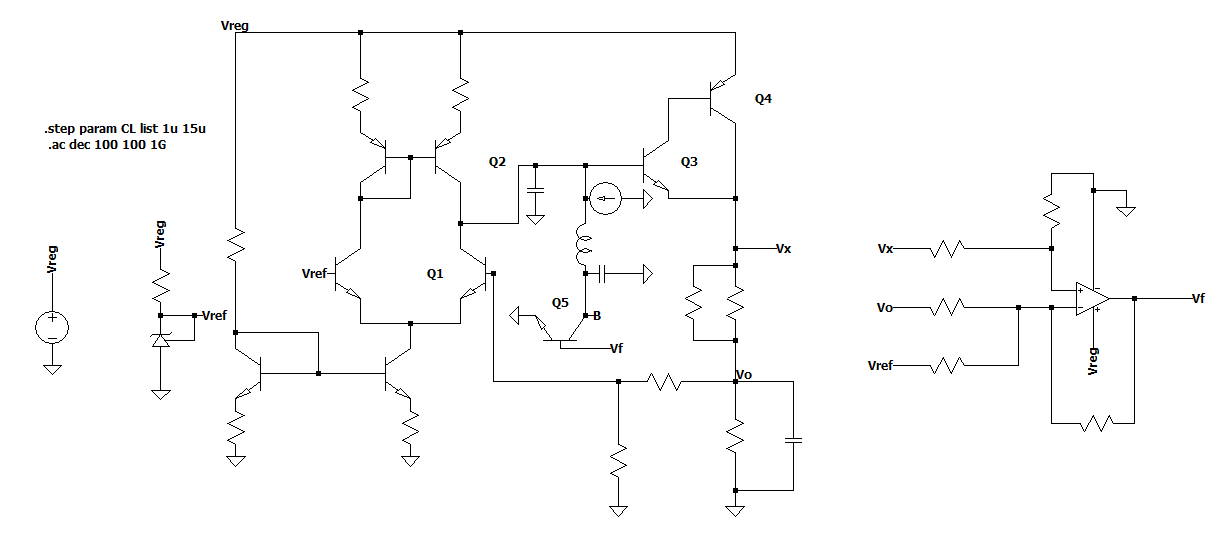
\includegraphics[width=0.9\linewidth]{img/Lazo de corriente/Circuito LC.png}
    \caption{Circutio utilizado para obtener el Bode del lazo de corriente}
    \label{fig:circuito LC}
\end{figure}

Nuevamente, el objetivo es hallar el bode de $L = a \cdot f$. Cabe aclarar que en el lazo de corriente el bloque $a$ son los transistores en configuración cuasi-darlington, mientras que el bloque $f$ está compuesto por la resistencia de sensado, el OpAmp y el transistor de drenaje. Por lo tanto, se abre el circuito entre la base de Q3 y el colector de Q5, se inyecta una corriente alterna y se toma la salida como la corriente del colector de Q5, indicado en la \autoref{fig:circuito LC} como nodo B. De esta forma, se obtuvo el bode de la \autoref{fig:LC sin compensar}. Nuevamente, se compensará el pero caso, que se produce para $C_L = \SI{1}{\micro \farad}$

\begin{figure}[H]
    \centering
    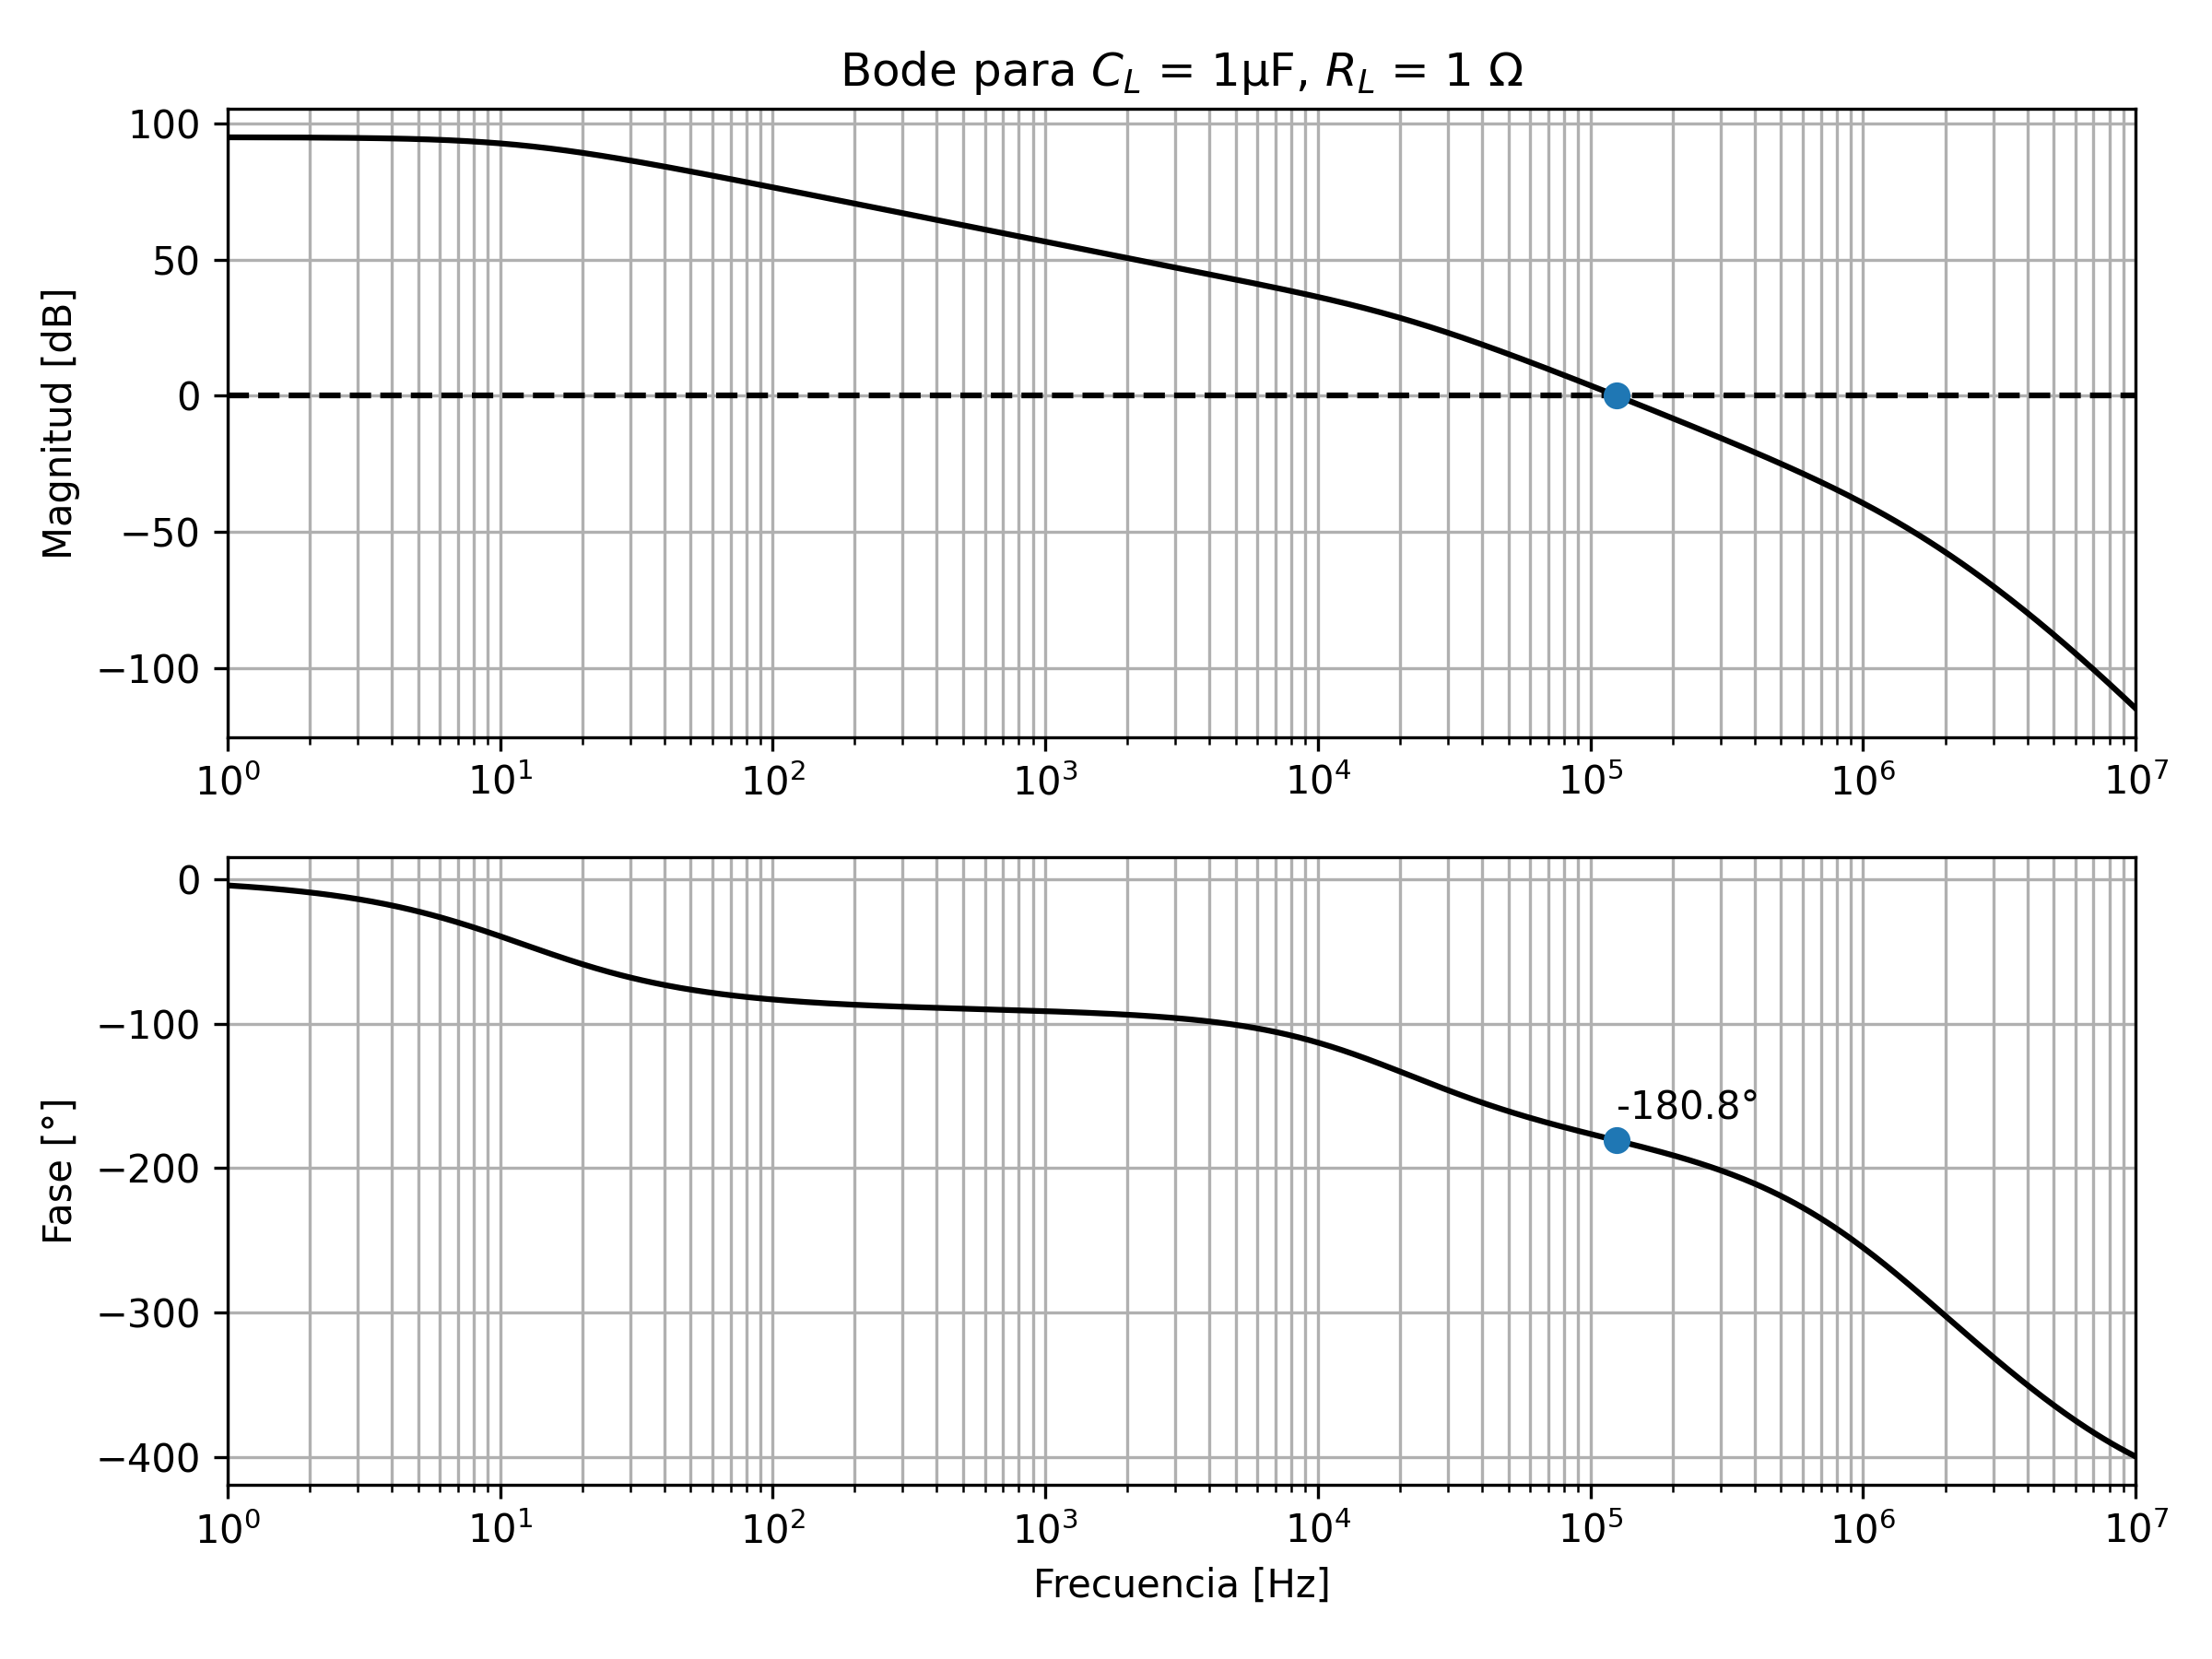
\includegraphics[width=0.9\linewidth]{img/Lazo de corriente/LC sin compensar.png}
    \caption{Lazo de corriente sin compensar}
    \label{fig:LC sin compensar}
\end{figure}

De este gráfico se concluye que es necesario añadir fase en las frecuencias del orden de los \SI{100}{\kilo \hertz}, por lo que debe añadirse un cero una década antes. Se añadirá entonces una resistencia en serie con el capacitor de \SI{330}{\nano \farad} ya agregado. De esta forma, se obtendría un cero en $z = \frac{1}{2\pi R C}$. De esta cuenta se despeja la resistencia para obtener un rango aproximado para la misma.

\begin{equation}
    R = \frac{1}{2\pi C z} = \frac{1}{2\pi \cdot \SI{330}{\nano \farad} \cdot \SI{10}{\kilo \hertz}} \approx  50 \Omega
\end{equation}

Por lo tanto, se necesita una resistencia del orden de las decenas de Ohm. Probando distintos valores comerciales, se obtiene que para $R = $ \SI{22}{\ohm} el lazo se estabiliza satisfactoriamente. En las Figuras \ref{fig: LC compensado CL=1uF}  y \ref{fig: LC compensado CL = 15uF} se muestran los diagrama de bode del lazo de corriente compensado para ambos casos de la capacidad de carga.

\begin{figure}[H]
    \centering
    
    \begin{subfigure}{0.9\textwidth}
        \centering
        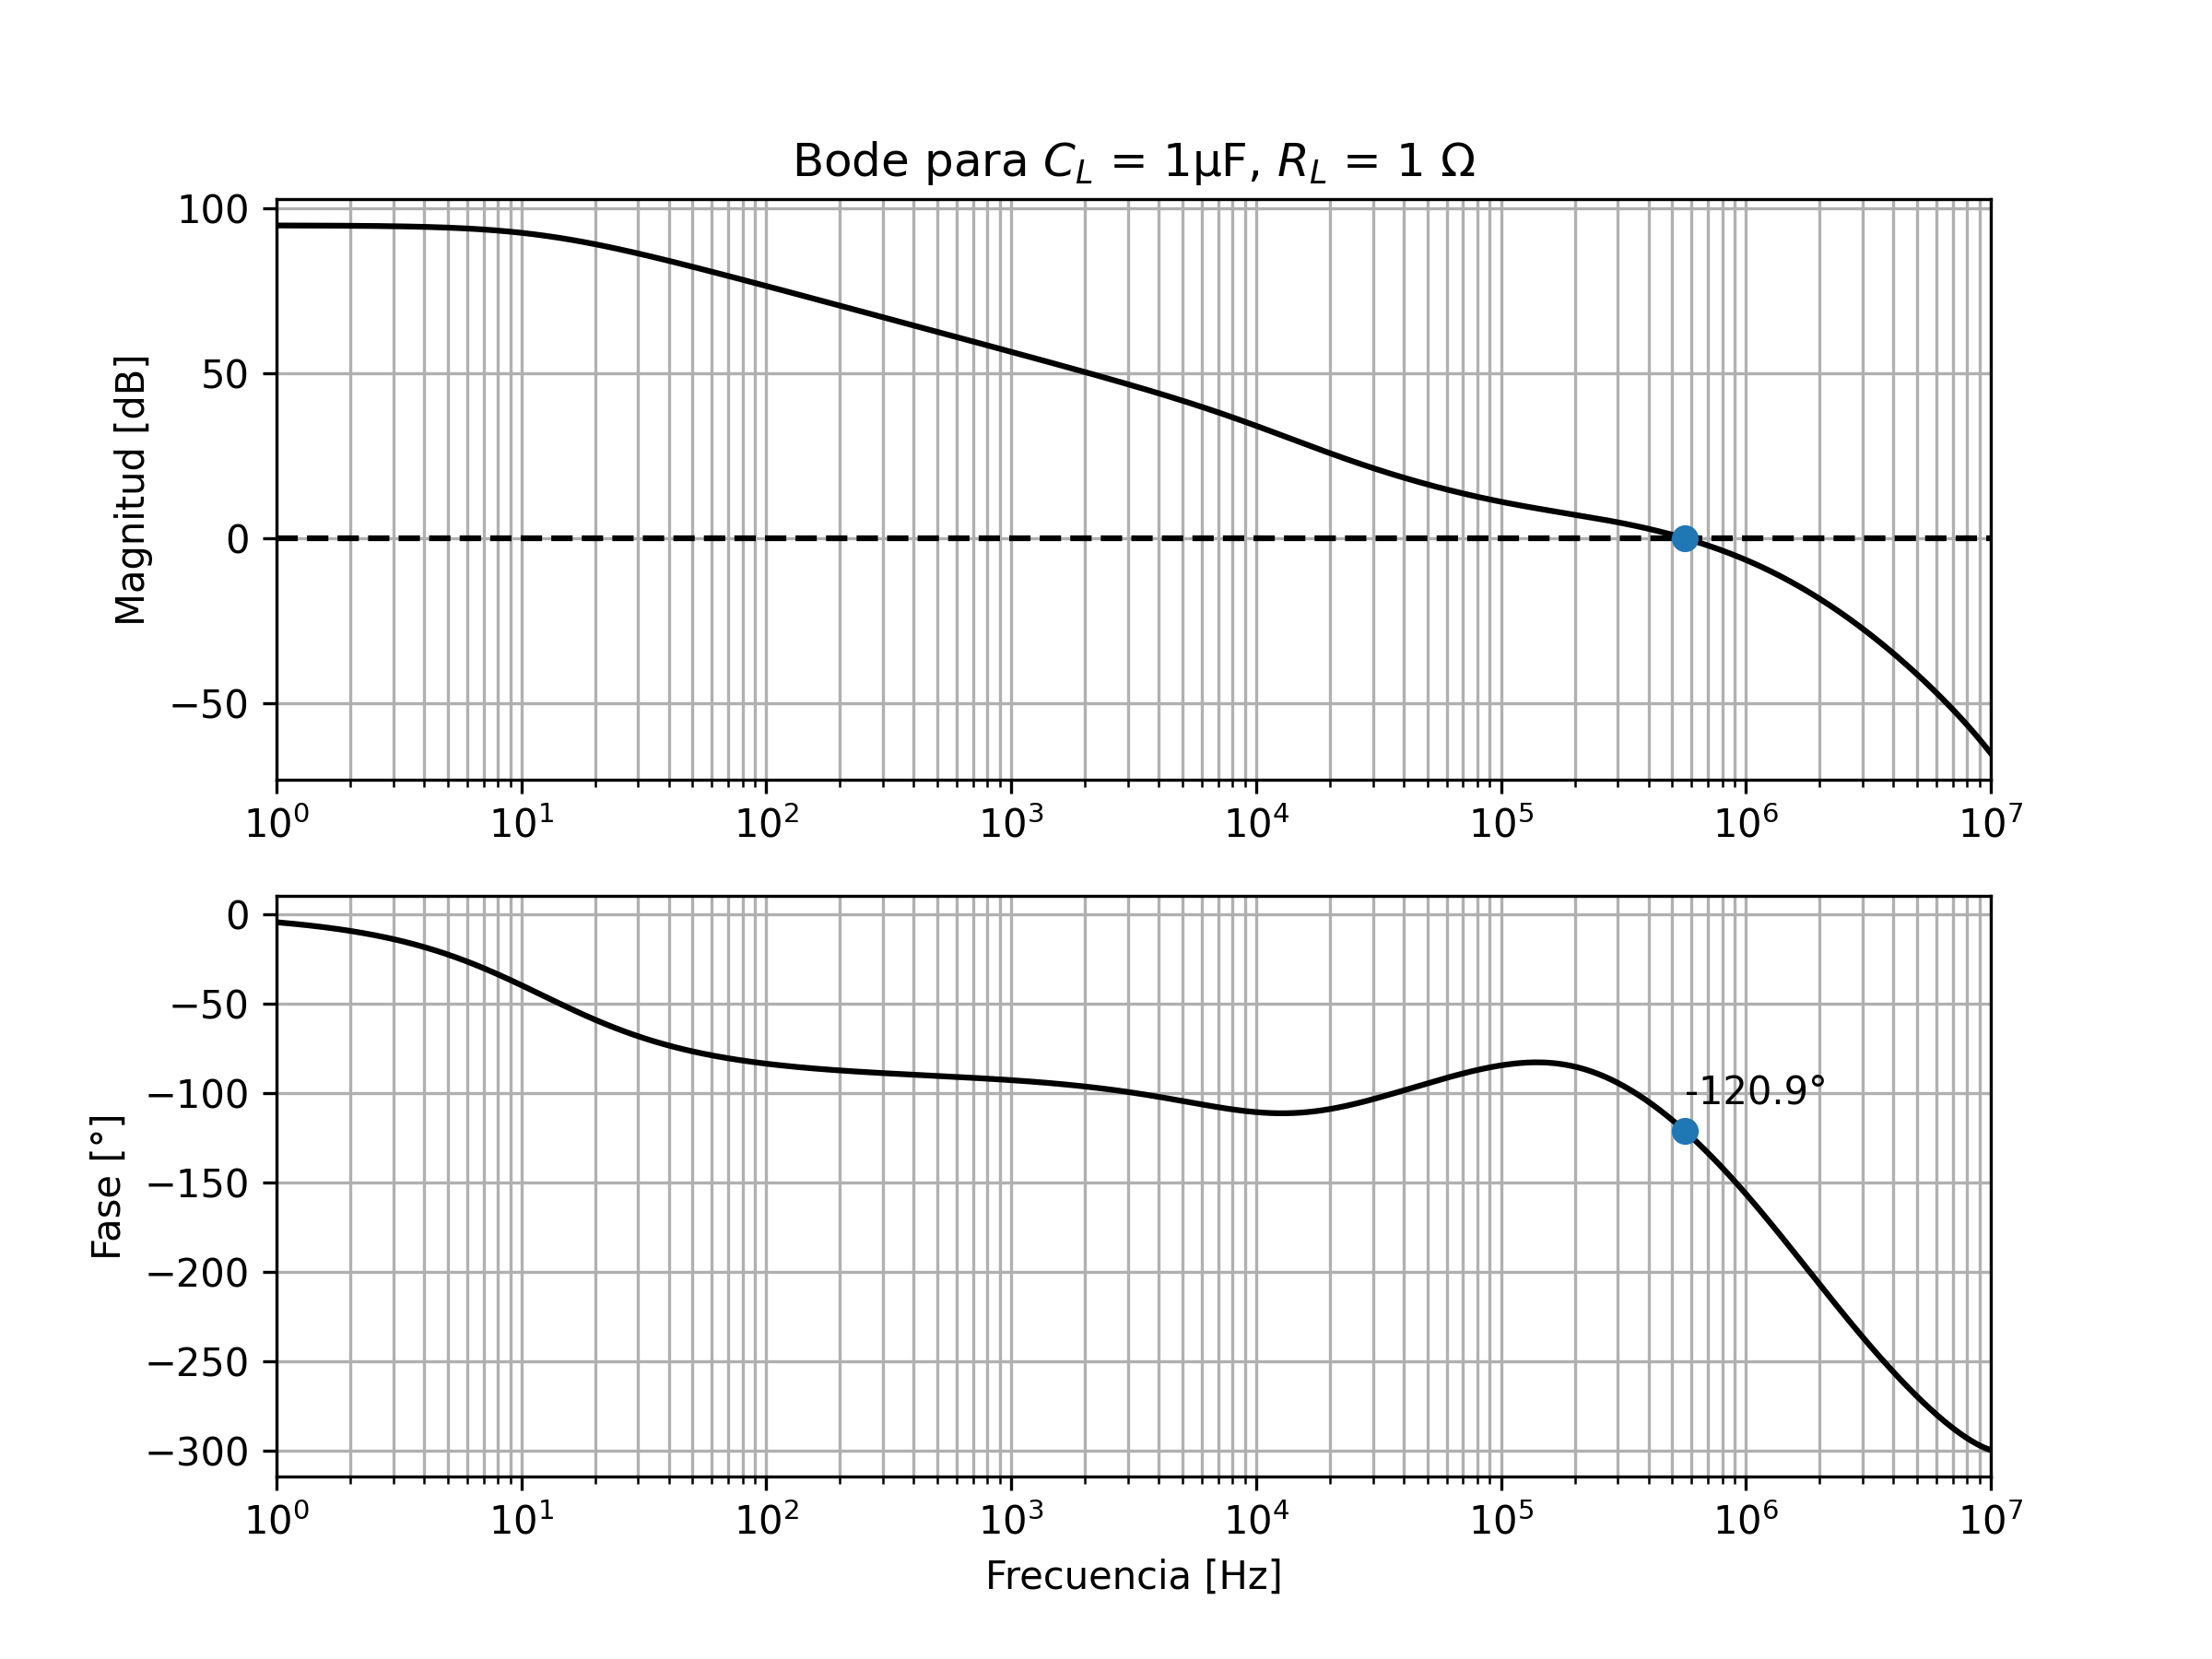
\includegraphics[width=\textwidth]{img/Lazo de corriente/LC compensado 1uF.png}
        \caption{Lazo de corriente compensado para $C_L = 1 \mu F$}
        \label{fig: LC compensado CL=1uF}
    \end{subfigure}
    
    \vspace{0.3cm}
    
    \begin{subfigure}{0.9\textwidth}
        \centering
        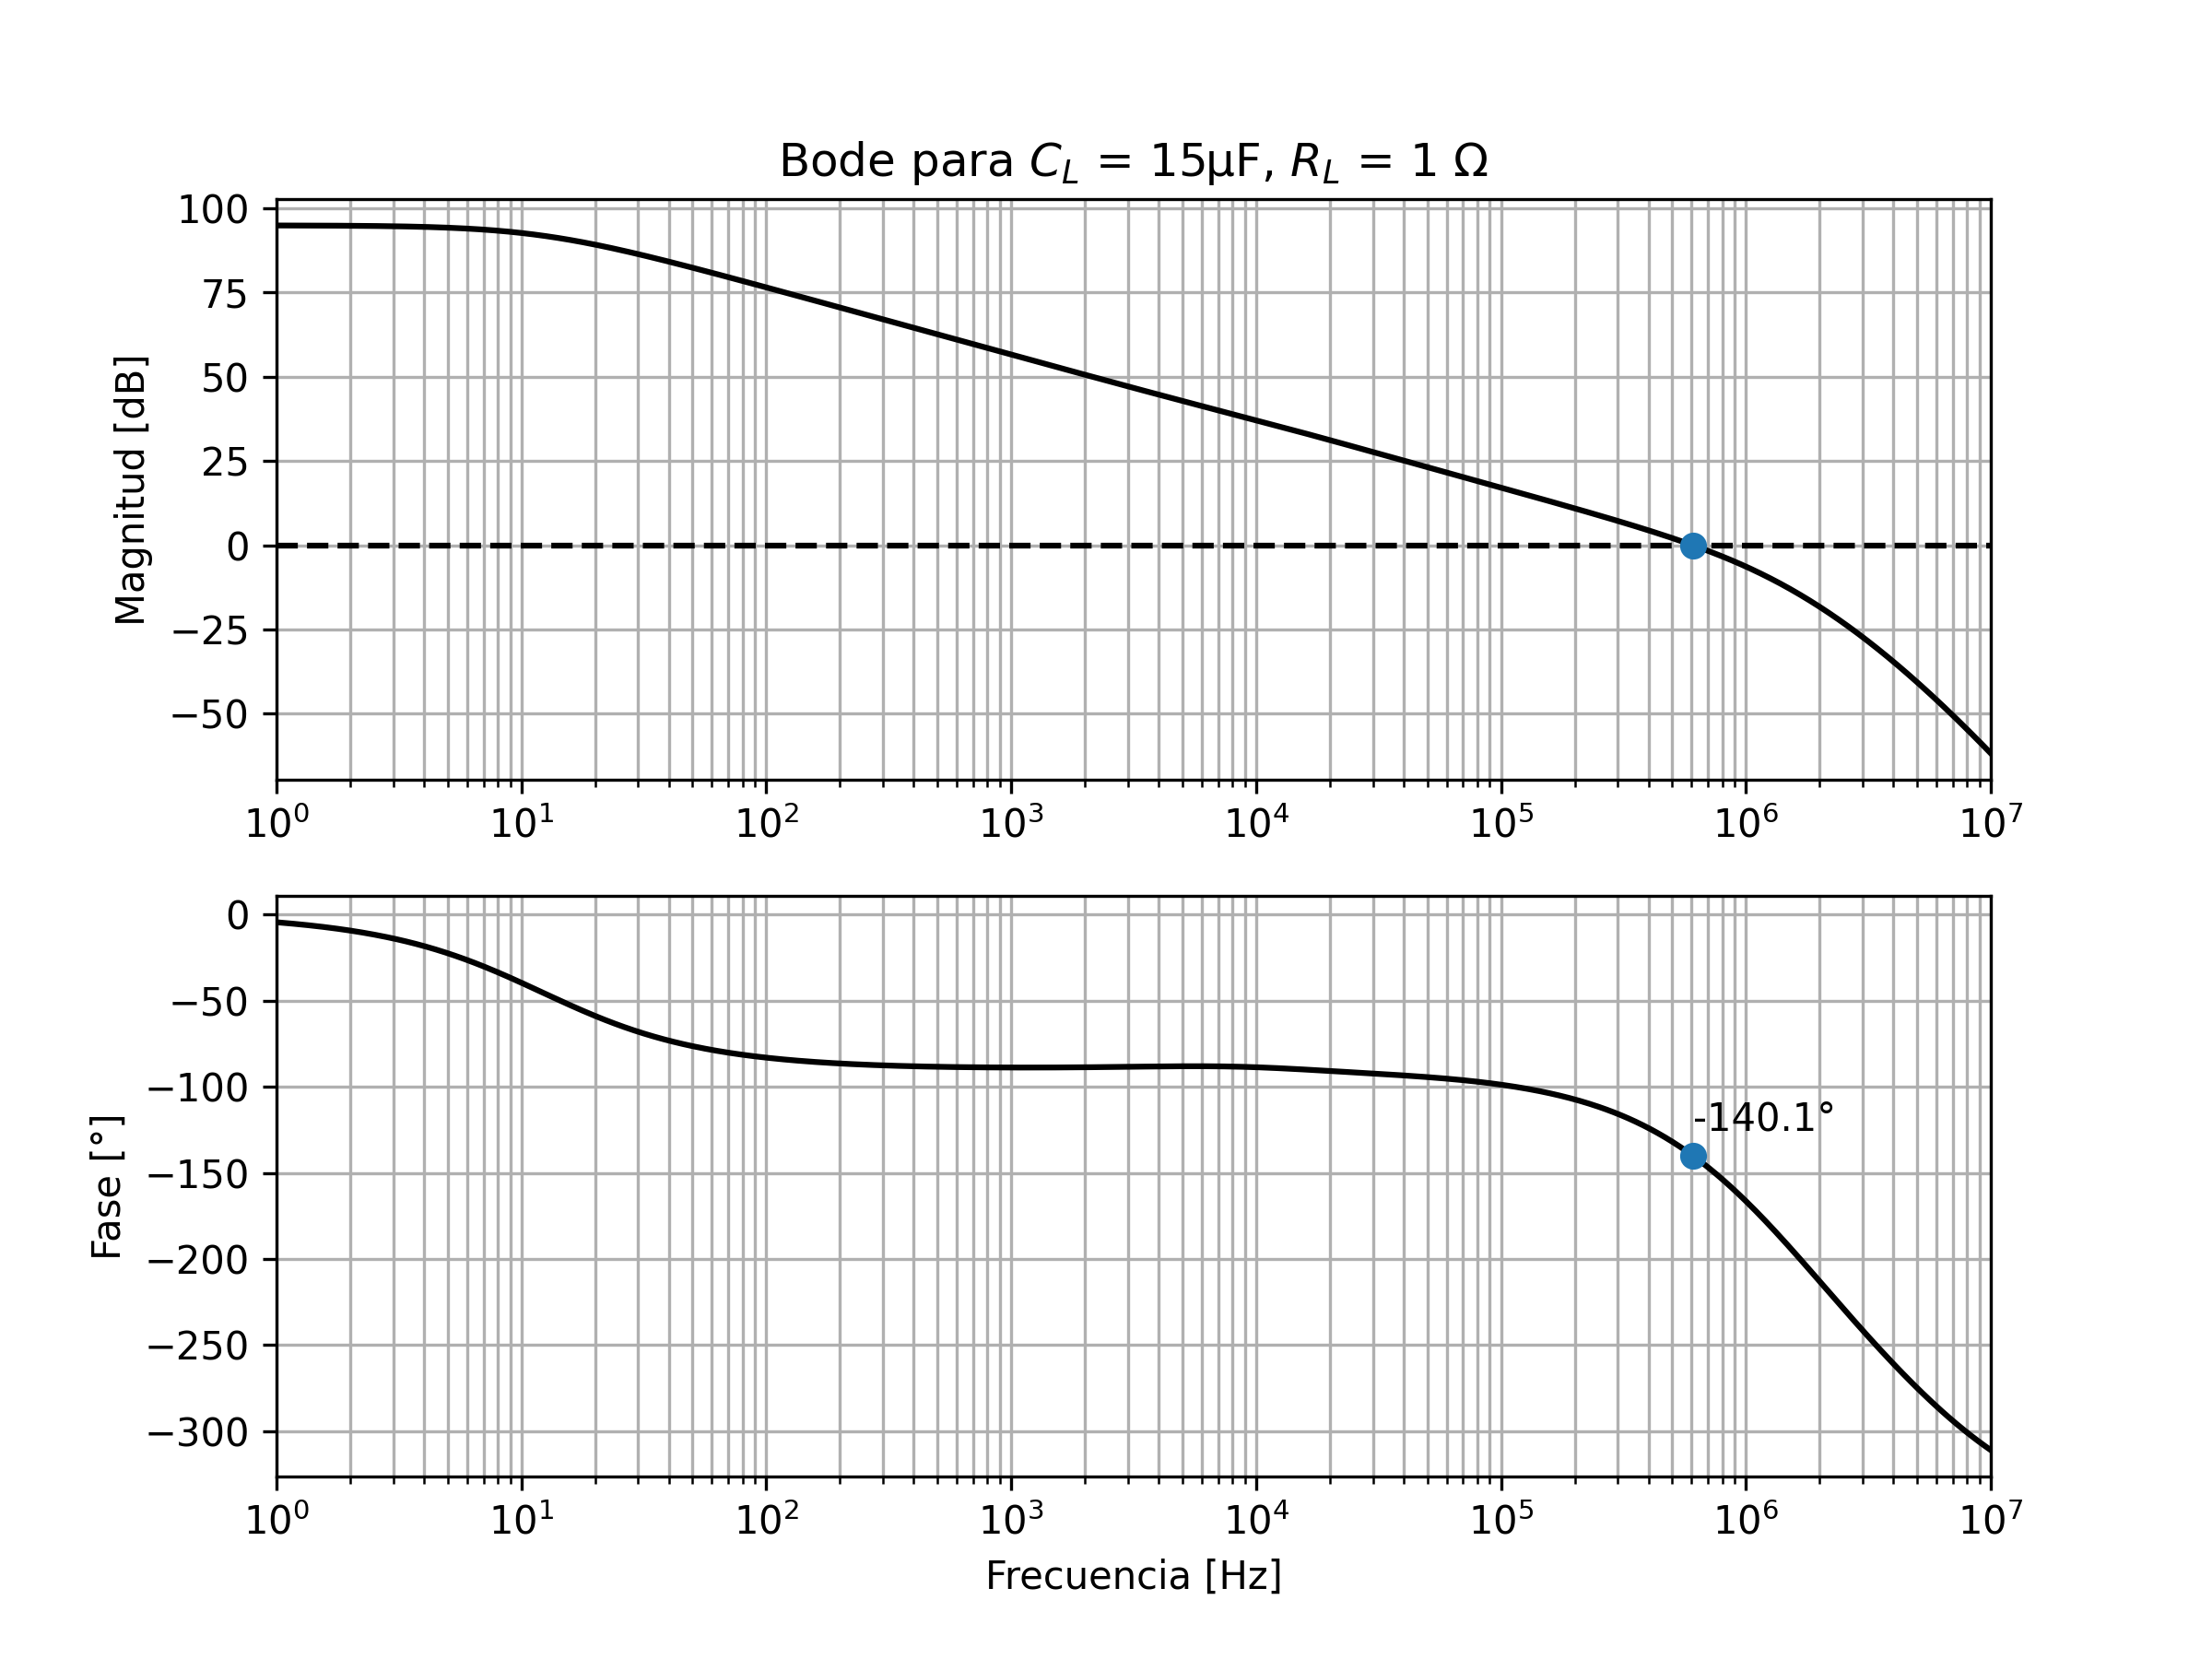
\includegraphics[width=\textwidth]{img/Lazo de corriente/LC compensado 15uF.png}
        \caption{Lazo de corriente compensado para $C_L = 15\mu F$}
        \label{fig: LC compensado CL = 15uF}
    \end{subfigure}
    
    \caption{Lazos de corriente compensados}
\end{figure}

Puede notarse que ahora, el pero caso se da para $C_L =  \SI{15}{\micro \farad} $. Finalmente, se simuló la respuesta al escalón para el circuito con y sin compensación. El circuito usado puede verse en la figura \ref{fig:circuito rta al escalon LC}

\begin{figure}[H]
    \centering
    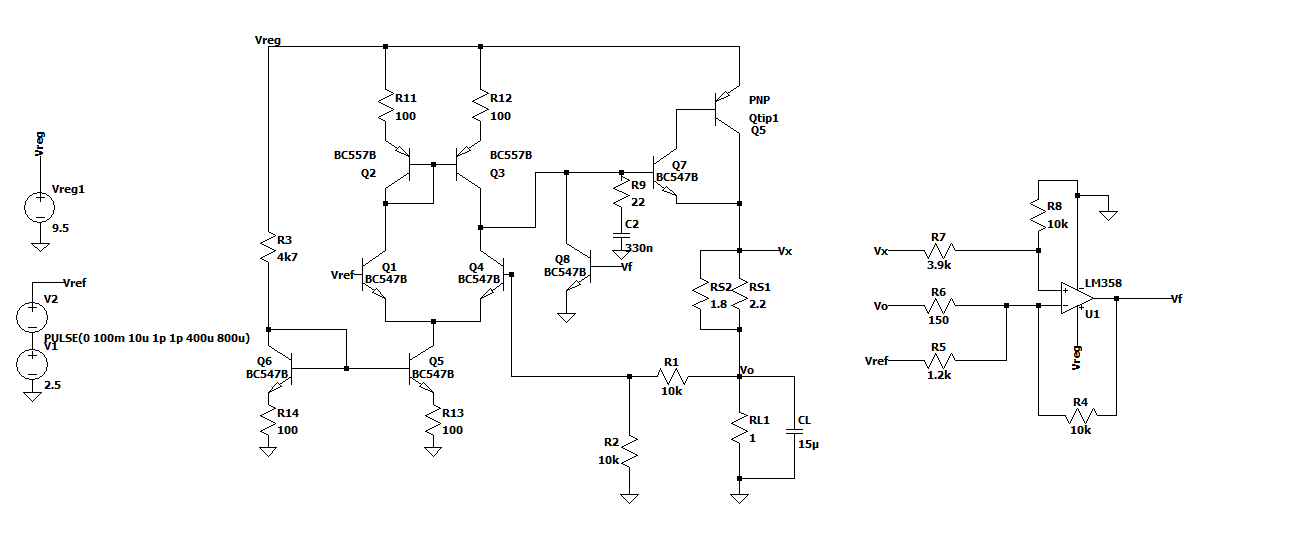
\includegraphics[width=0.9\linewidth]{img/Lazo de corriente/Circuito LC rta al escalon.png}
    \caption{Circuito utilizado para medir la respuesta al escalón}
    \label{fig:circuito rta al escalon LC}
\end{figure}

\begin{figure}[h]
    \centering

    \begin{subfigure}{0.45\textwidth}
        \centering
        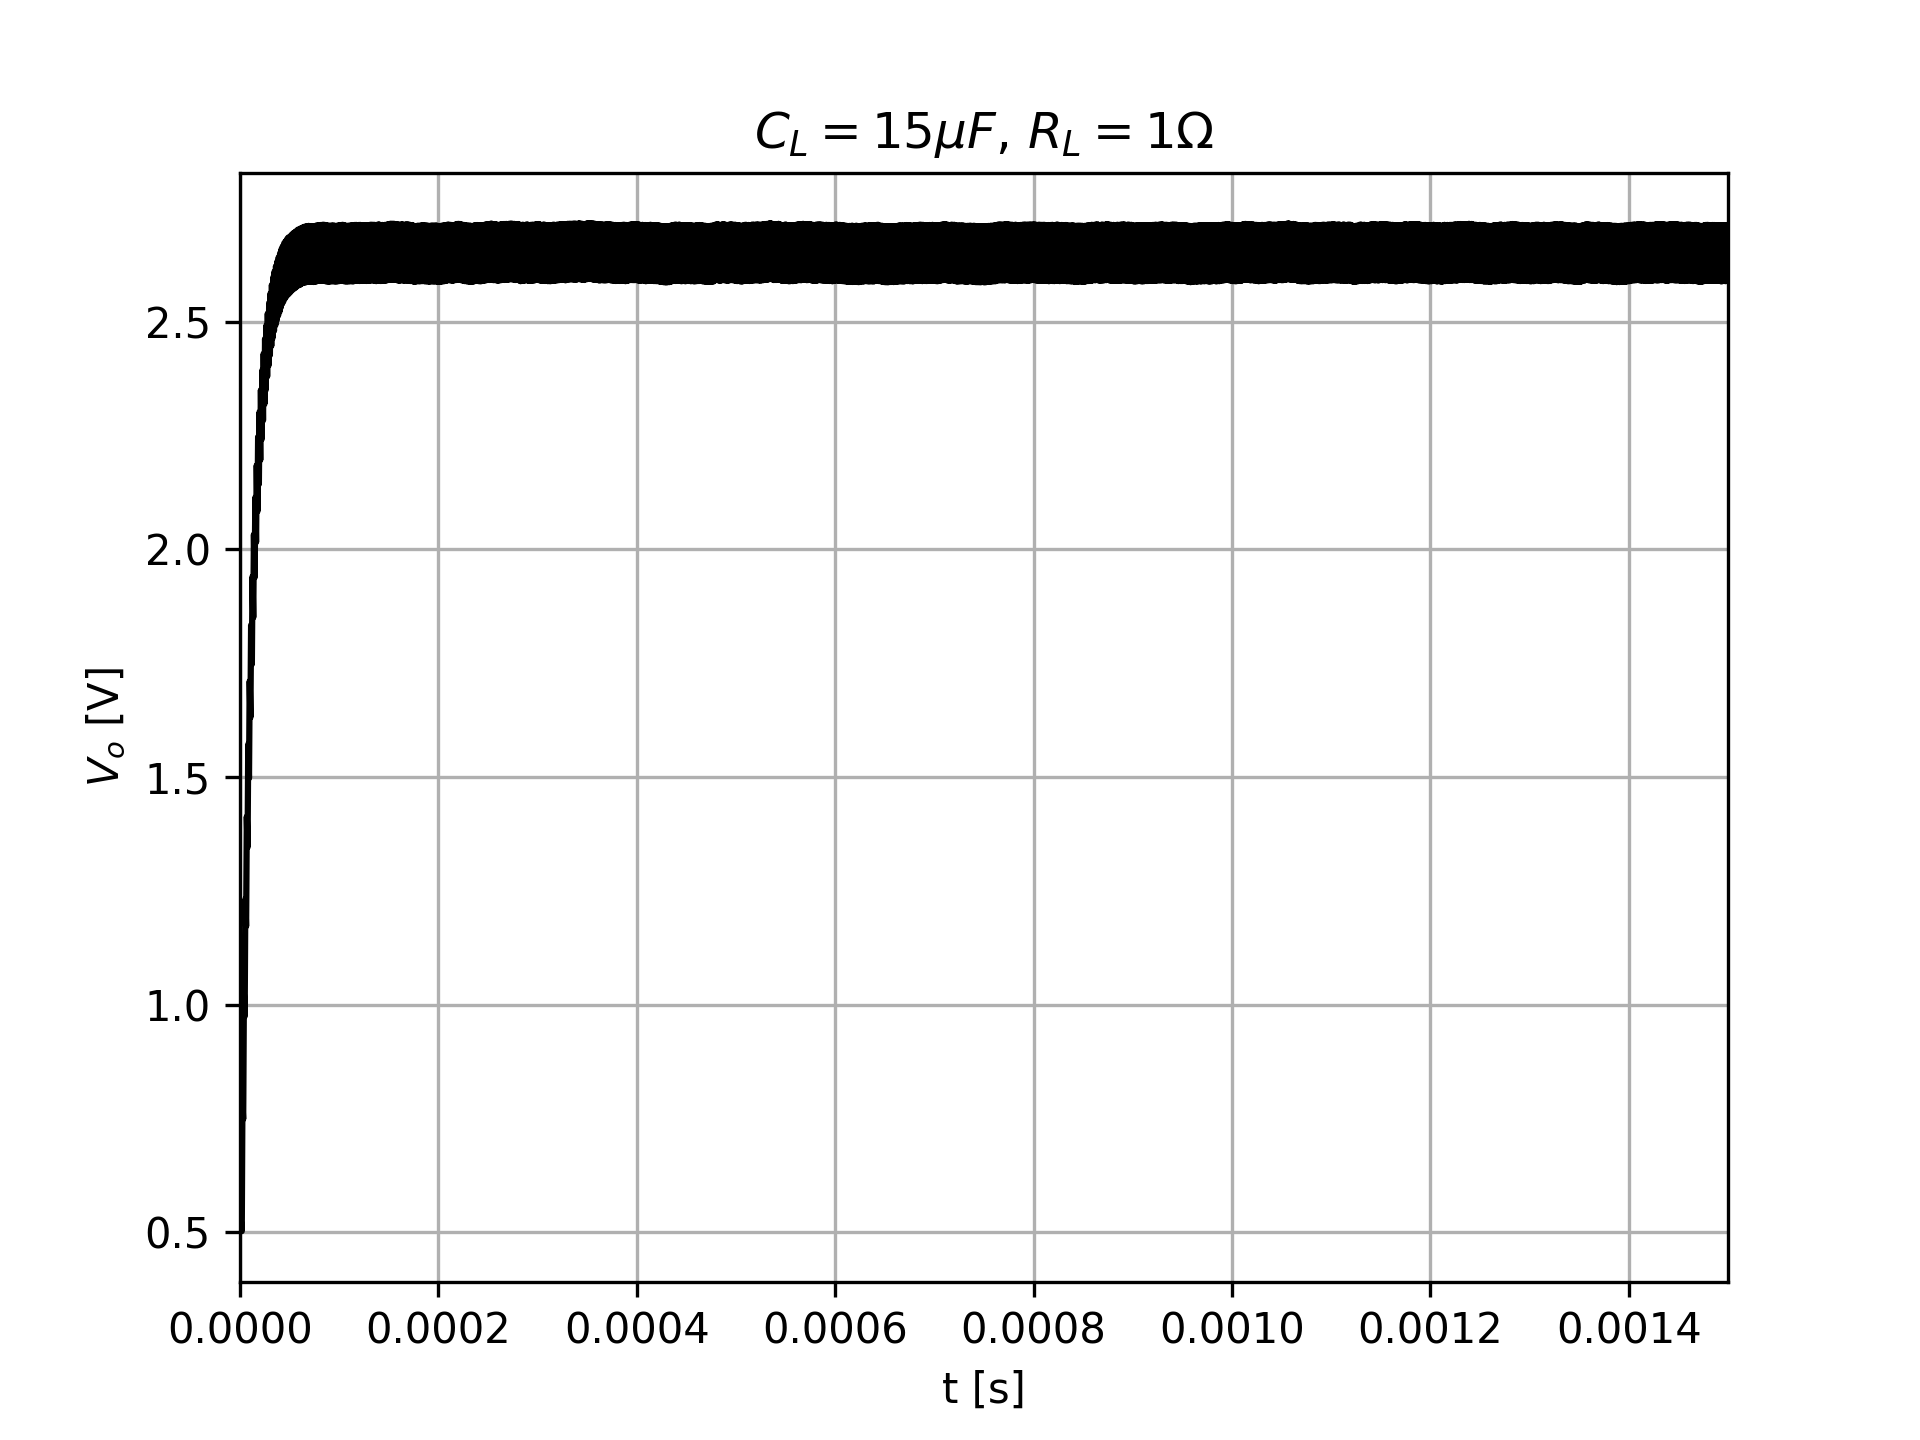
\includegraphics[width=\linewidth]{img/Lazo de corriente/Rta al escalon LC (sin compensar).png}
        \caption{Respuesta al escalón sin compensar}
    \end{subfigure}
    \hfill
    \begin{subfigure}{0.45\textwidth}
        \centering
        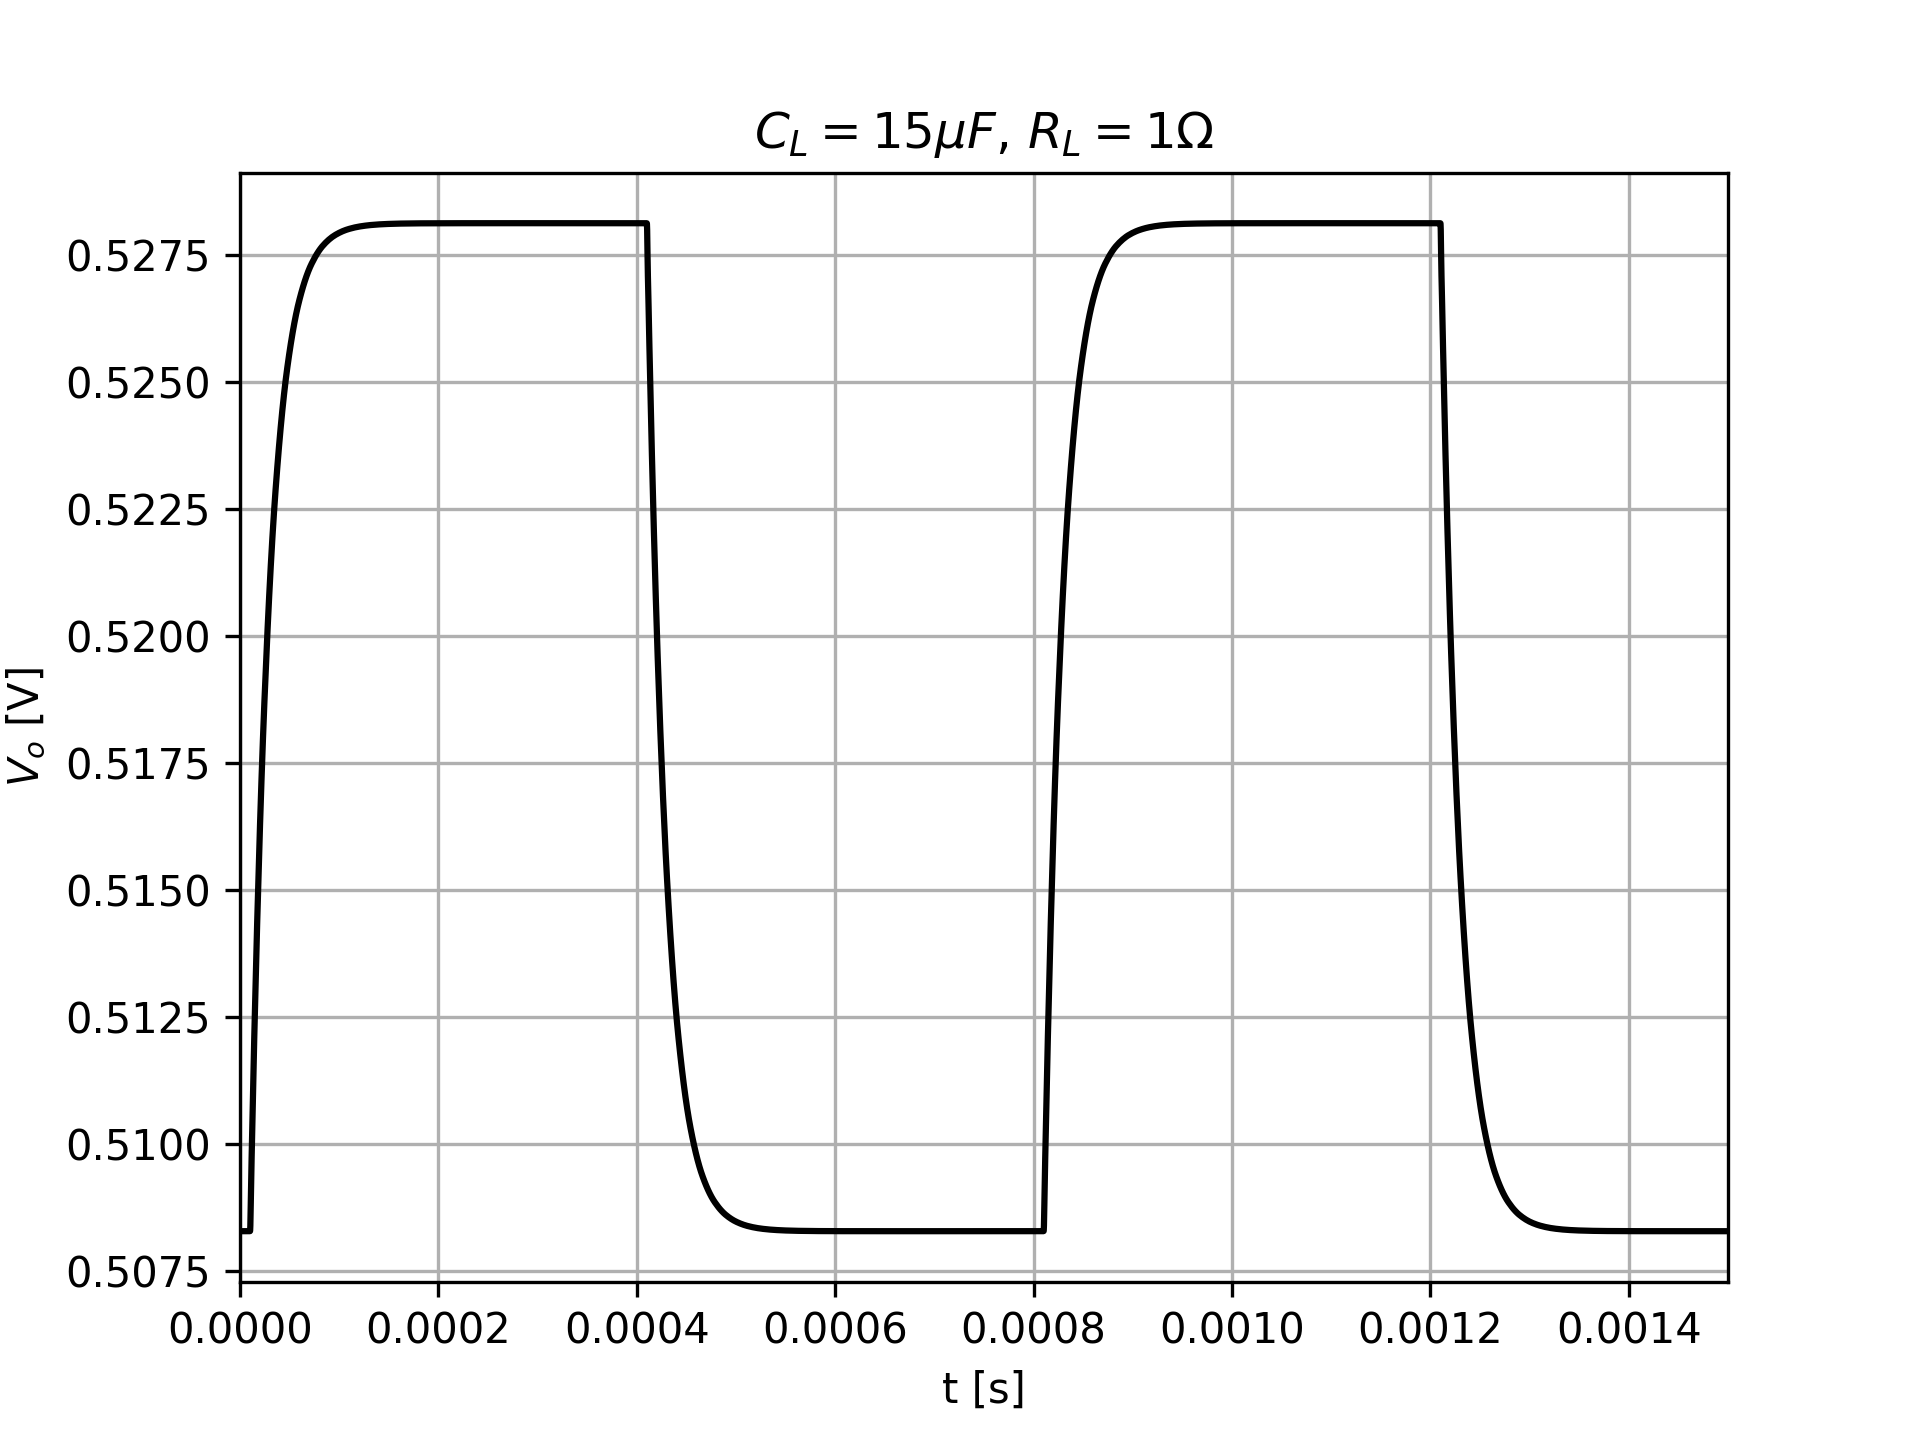
\includegraphics[width=\linewidth]{img/Lazo de corriente/Rta al escalon LC(compensada).png}
        \caption{Respuesta al escalón compensada}
    \end{subfigure}

    \caption{Respuestas al escalón}
\end{figure}